% Ergebnisse und Analyse.tex

% Ergebnisse und Analyse Diagramme.tex

\newcommand{\MergesortMesswerte}{%
    \addplot[blue, mark=*] coordinates {
            (25000000,3017372600)
            (50000000,6315632400)
            (100000000,12777405700)
            (200000000,27203738300)
            (400000000,56441153000)
        };
    \addlegendentry{Mergesort}
}

\newcommand{\QuicksortMesswerte}{%
    \addplot[green, mark=*] coordinates {
            (25000000,1528071600)
            (50000000,3248990900)
            (100000000,6653966800)
            (200000000,13778762100)
            (400000000,29074726600)
        };
    \addlegendentry{Quicksort}
}

\newcommand{\GrundlegendeLaufzeitenAbhaengigVonDerArraygroesseDiagrammA}{%
    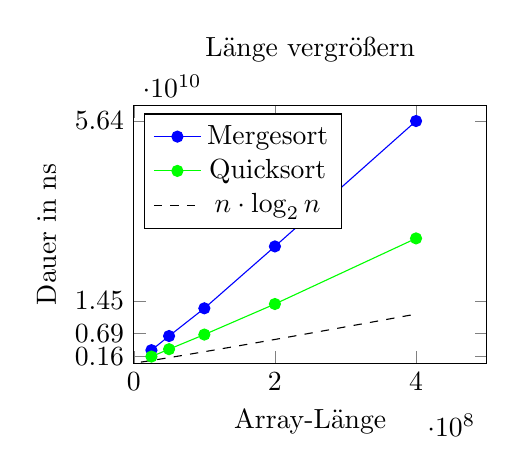
\begin{tikzpicture}
        \begin{axis}[
                title style={yshift=1.5ex},
                width=0.5\textwidth,
                height=0.4\textwidth,
                xlabel={Array-Länge},
                ylabel={Dauer in ns},
                title={Länge vergrößern},
                xmin=0, xmax=5 * 10^8,
                ymin=0*10^6, ymax=6*10^10,
                grid style=dashed,
                legend pos=north west,
                ytick={1609541400,6854920900,14495472700,56441153000},
                % xtick={2^21,2^23,2^24,2^25},
                % xticklabels={$2^{21}$, $2^{23}$, $2^{24}$, $2^{25}$},
                % scaled x ticks=false,
                % scaled y ticks=false,
            ]
            \MergesortMesswerte
            \QuicksortMesswerte
            % n*log2(n)
            \addplot[black, dashed,domain=1e7:4e8, samples=100] {x*log2(x)};
            \addlegendentry{$n \cdot \log_2 n$}
            % % n
            % \addplot[red, dashed,domain=1e7:4e8, samples=100] {x};
            % \addlegendentry{$n$}
            % % log2(n)
            % \addplot[green, domain=1e7:4e8, samples=100] {log2(x)};
            % \addlegendentry{$\log_2 n$}
        \end{axis}
    \end{tikzpicture}%
}

\newcommand{\GrundlegendeLaufzeitenAbhaengigVonDerArraygroesseDiagrammB}{%
    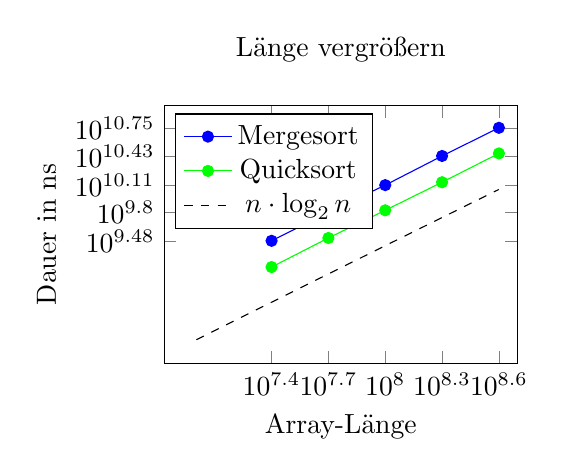
\begin{tikzpicture}
        \begin{axis}[
                title style={yshift=1.5ex},
                width=0.5\textwidth,
                height=0.4\textwidth,
                xlabel={Array-Länge},
                ylabel={Dauer in ns},
                title={Länge vergrößern},
                xmin=0, xmax=5 * 10^8,
                ymin=0*10^6, ymax=1*10^11,
                grid style=dashed,
                legend pos=north west,
                xmode=log,
                log basis x=10,
                xtick=data,
                ymode=log,
                log basis y=10,
                ytick=data,
                % xtick={2^21,2^23,2^24,2^25},
                % xticklabels={$2^{21}$, $2^{23}$, $2^{24}$, $2^{25}$},
                % scaled x ticks=false,
                % scaled y ticks=false,
            ]
            \MergesortMesswerte
            \QuicksortMesswerte
            % n*log2(n)
            \addplot[black, dashed,domain=1e7:4e8, samples=100] {x*log2(x)};
            \addlegendentry{$n \cdot \log_2 n$}
        \end{axis}
    \end{tikzpicture}%
}


% Definiere Variablen
% \newcommand{\Messziel}{Messziel}

% % ----------------------
% % 4. Ergebnisse und Analyse
% % ----------------------
% \newpage
% \chapter{Ergebnisse und Analyse}
% \paragraph{Hinweis zum Umfang der Darstellung}
% \section{Grundlegende Laufzeiten abhängig von der Arraygröße}
% \subsection{Messziel} % Einleitung
% \subsection{Erwartung}
% \subsection{Diagramm}
% \subsection{Analyse und Interpretation}
% \newpage
% \section{Einfluss des Listentyps} % Listentyps: Zufall, Sortiert, InvertiertSortiert, FastSortiert, Dupliziert
% \subsection{Messziel} % Einleitung
% \subsection{Erwartung}
% \subsection{Diagramm}
% \subsection{Analyse und Interpretation}
% \newpage
% \section{Einfluss der Arraygröße im Detail}
% \subsection{Messziel} % Einleitung
% \subsection{Erwartung}
% \subsection{Diagramm}
% \subsection{Analyse und Interpretation}
% \newpage
% \section{Tiefenbasierte Thread-Erzeugung}
% \subsection{Messziel} % Einleitung
% \subsection{Erwartung}
% \subsection{Diagramm}
% \subsection{Analyse und Interpretation}
% \newpage
% \section{Workerthreads}
% \subsection{Messziel} % Einleitung
% \subsection{Erwartung}
% \subsection{Diagramm}
% \subsection{Analyse und Interpretation}
% \newpage
% \section{Vergleich der Threading-Methoden}
% \subsection{Messziel} % Einleitung
% \subsection{Erwartung}
% \subsection{Diagramm}
% \subsection{Analyse und Interpretation}
% \newpage
% \section{Einfluss des Datentyps der Liste} % Listenart: int, string
% \subsection{Messziel} % Einleitung
% \subsection{Erwartung}
% \subsection{Diagramm}
% \subsection{Analyse und Interpretation}
% % \section{Debug Vs Release}

% % ----------------------
% % 4. Ergebnisse und Analyse
% % ----------------------
% \chapter{Ergebnisse und Analyse}
% \paragraph{Hinweis zum Umfang der Darstellung}
\newcommand{\HinweisZumUmfangDerDarstellung}{
    Alle beschriebenen Messungen wurden vollständig durchgeführt und die
    entsprechenden Rohdaten liegen vor. Aufgrund des begrenzten zeitlichen
    Rahmens dieser Bachelorarbeit wird jedoch auf eine vollständige grafische
    Darstellung sowie eine detaillierte Analyse aller Messreihen verzichtet.
    Stattdessen werden im Folgenden ausgewählte, repräsentative Messungen
    dargestellt und analysiert, da diese ausreichend sind, um die theoretisch
    erwarteten Laufzeiteigenschaften der untersuchten Algorithmen zu bestätigen.
    Weitere Messdaten würden keine zusätzlichen inhaltlichen Erkenntnisse liefern,
    sondern lediglich bereits beobachtete Effekte wiederholen.
}

% \section{Grundlegende Laufzeiten abhängig von der Arraygröße}
% \subsection{Messziel} % Einleitung
\newcommand{\GrundlegendeLaufzeitenAbhaengigVonDerArraygroesseMessziel}{
    Das Messziel besteht darin, die Abhängigkeit der sequenziellen Implementierungen von der Arraygröße grafisch darzustellen.
    Dadurch können diese Ergebnisse später mit den parallelen Varianten verglichen werden.
    Gleichzeitig dient dies als einfacher Einstieg in das Thema.
}

% \subsection{Erwartung}
\newcommand{\GrundlegendeLaufzeitenAbhaengigVonDerArraygroesseErwartung}{
    Da die durchschnittliche Laufzeit \(O(n \log n)\) beträgt, wird eine logarithmische Laufzeiterhöhung bei wachsender Arraygröße erwartet.
}

% \subsection{Diagramm}
\newcommand{\GrundlegendeLaufzeitenAbhaengigVonDerArraygroesseDiagramm}{
    \GrundlegendeLaufzeitenAbhaengigVonDerArraygroesseDiagrammA
    \GrundlegendeLaufzeitenAbhaengigVonDerArraygroesseDiagrammB
    \newline
    \GrundlegendeLaufzeitenAbhaengigVonDerArraygroesseDiagrammC
}

% \subsection{Analyse und Interpretation}
\newcommand{\GrundlegendeLaufzeitenAbhaengigVonDerArraygroesseAnalyse}{
    In den ersten zwei Diagrammen ist die Veränderung der Laufzeit zu sehen, wenn die Listengröße fünfmal verdoppelt wird und bei \(2.5 \cdot 10^7\) startet.
    Beim zweiten Diagramm sind die Achsen logarithmisch dargestellt, da dies die Darstellung und den Vergleich der Laufzeiten erleichtert.
    \newline
    Unter diesen beiden Diagrammen befindet sich ein drittes Diagramm, in dem die gemessenen Laufzeiten ebenfalls logarithmisch dargestellt sind und der Größenbereich von \(1\) bis \(800\,000\) betrachtet wird.
    \newline
    Anhand dieser Diagramme ist deutlich erkennbar, dass sowohl Mergesort als auch Quicksort tatsächlich eine Laufzeit von
    \(O(n \log n)\) besitzen.
    \newline
    Zudem ist erkennbar, dass Mergesort etwa doppelt so lange benötigt wie Quicksort und dass Quicksort näherungsweise eine Laufzeit von
    \(2 \cdot n \log_2(n)\) aufweist.
    \newline
    Da eine lineare Laufzeit auf einen Blick leichter zu interpretieren ist, wurde zusätzlich die Funktion \(32n\) eingezeichnet.
    Anhand dieser Funktion ist erkennbar, dass sie im untersuchten Zahlenbereich von \(1\) bis \(4 \cdot 10^8\) teilweise sogar eine genauere Abschätzung liefert als \(n \log_2(n)\).
    Daraus folgt, dass von einer gerundeten Mindestlaufzeit von \(32n\) ausgegangen werden kann.
    \newline
    Abschließend ist anzumerken, dass alle Messungen mit einer Laufzeit von kleiner oder gleich \(10^4\,\text{ns}\) aufgrund der Messtoleranz nur eine eingeschränkte Aussagekraft besitzen.
    Zwar kann mit \texttt{chrono} auf eine Auflösung von \(100\,\text{ns}\) genau gemessen werden, dennoch verbleiben natürliche Schwankungen, die insbesondere im Bereich von \(10^4\,\text{ns}\) einen erheblichen Einfluss auf die Messergebnisse haben.
}

% \section{Einfluss des Listentyps} % Listentyps: Zufall, Sortiert, InvertiertSortiert, FastSortiert, Dupliziert
% \subsection{Messziel} % Einleitung
\newcommand{\EinflussDesListentypsMessziel}{
    Der Listentyp ist relevant, da Quicksort sowohl einen Best-Case als auch einen Worst-Case aufweist.
    Diese hängen vom Inhalt der zu sortierenden Liste und somit vom jeweiligen Listentyp ab.
    Gleichzeitig dient diese Messung der Vollständigkeit, sodass die Laufzeiten auch mit anderen,
    nicht in dieser Arbeit implementierten Sortieralgorithmen gut vergleichbar sind.
    Auch hierbei werden zunächst ausschließlich die seriellen Laufzeiten der Algorithmen gemessen.
    Zur Vollständigkeit werden zusätzlich weitere Listentypen außer zufällig und sortiert betrachtet.
}

% \subsection{Erwartung}
\newcommand{\EinflussDesListentypsErwartung}{
    Es wird erwartet, dass der Listentyp bei Mergesort nahezu keinen Einfluss auf die Laufzeit hat,
    sodass lediglich sehr geringe Laufzeitänderungen zu beobachten sind.
    Für Quicksort wird bei einer sortierten Liste der Best-Case erwartet,
    da als Pivotelement jeweils das mittlere Element gewählt wird.
    Ebenso wird erwartet, dass bei Quicksort bei Wahl des jeweils rechten Elements als Pivotelement
    bei einer sortierten Liste der Worst-Case eintritt.
}

% \subsection{Diagramm}
\newcommand{\EinflussDesListentypsDiagramm}{
    \EinflussDesListentypsDiagrammA
    \newline
    \EinflussDesListentypsDiagrammB
    \newline
    \EinflussDesListentypsDiagrammC
}

% \subsection{Analyse und Interpretation}
\newcommand{\EinflussDesListentypsAnalyse}{
    Die gemessenen Daten zeigen deutlich, dass der Best-Case von Quicksort in der Praxis besser als \(n \log_2(n)\) ausfällt.
    Dies ist darauf zurückzuführen, dass die Messungen in der Release-Version mit aktivierten Compiler-Optimierungen durchgeführt wurden.
    In der Debug-Version (ohne Compiler-Optimierungen) wurde bei einem sortierten Array der Größe von 400~Millionen Elementen
    hingegen eine Laufzeit von 14~s für Quicksort gemessen, welche oberhalb der erwarteten Laufzeit von \(n \log_2(n)\) liegt.
    Die Messungen zeigen außerdem, dass sortierte, invertiert sortierte sowie fast sortierte Arrays nahezu identische Laufzeiten aufweisen.
    Die entsprechenden Kurven würden nahezu übereinanderliegen, weshalb zugunsten der Übersichtlichkeit auf eine separate grafische Darstellung
    dieser Listentypen verzichtet wurde.
    Im Diagramm ist ebenfalls zu erkennen, dass der Worst-Case von Quicksort eine Laufzeit von \(O(n^2)\) besitzt.
    Allerdings endet der Graph ab 20k, da bereits bei 40k ein Stackoverflow durch die Rekursionstiefe ausgelöst wird. Dies ließe sich durch eine iterative Version von Quicksort vermeiden.
}

% \section{Tiefenbasierte Thread-Erzeugung}
% \subsection{Messziel} % Einleitung
% \subsection{Erwartung}
% \subsection{Diagramm}
% \subsection{Analyse und Interpretation}

% \section{Tiefenbasierte Thread-Erzeugung}
% \subsection{Messziel} % Einleitung
\newcommand{\TiefenbasierteThreadErzeugungMessziel}{
    Hier wird die rekursive Variante gemessen, die einen der beiden rekursiven Selbstaufrufe in einem neuen Thread ausführt.
    Dabei gibt es jedoch ein Limit, da jeder Thread selbst Speicher benötigt und der RAM nicht unendlich groß ist.
    Hierbei soll gemessen werden, welchen Performance-Unterschied eine höhere Anzahl an Threads bewirkt.
}

% \subsection{Erwartung}
\newcommand{\TiefenbasierteThreadErzeugungErwartung}{
    Es wird ein theoretisch linearer Performance-Zuwachs erwartet, solange kein Hardware-Limit erreicht wird.
    Zudem wird in dieser Variante erwartet, dass Mergesort besser skaliert als Quicksort,
    da Quicksort die Liste nicht exakt in der Mitte teilt, sondern dies nur theoretisch im Durchschnitt tut.
    Der Best Case von Quicksort sollte jedoch weiterhin wesentlich besser sein als der von Mergesort,
    da Quicksort in diesem Fall die Liste immer perfekt in der Mitte teilt.
    Außerdem wird erwartet, dass sich die Laufzeit deutlich verschlechtert, wenn mehr Threads genutzt werden als logische Prozessoren vorhanden sind,
    da der Overhead durch Thread-Initialisierung und Context-Switching zunimmt.
}

% \subsection{Diagramm}
\newcommand{\TiefenbasierteThreadErzeugungDiagramm}{
    \TiefenbasierteThreadErzeugungDiagrammB
    \newline
    \TiefenbasierteThreadErzeugungDiagrammC
    \newline
    \TiefenbasierteThreadErzeugungDiagrammA
}
% \subsection{Analyse und Interpretation}
\newcommand{\TiefenbasierteThreadErzeugungAnalyse}{
    Entgegen der ursprünglichen Erwartung konnte kein signifikanter Performance Unterschied zwischen einer vollständig sortierten und einer nahezu sortierten Liste bei Quicksort festgestellt werden.
    Dieses Verhalten ist vermutlich auf Compiler-Optimierungen zurückzuführen und darauf, dass in der Implementierung nicht systematisch ein besonders ungünstiges Pivot-Element gewählt wurde.
    \newline
    Deutliche Performance-Verbesserungen sind jedoch in allen Bereichen messbar, wie theoretisch zu erwarten war.
    Für ein unsortiertes Array der Größe \(400 \, \text{Mio.}\) zeigt sich, dass Mergesort mit 16 Threads lediglich etwa 16~\% der Laufzeit der seriellen Variante benötigt, während Quicksort 26~\% erreicht.
    Die Laufzeit von Mergesort wächst dabei sehr regelmäßig, während Quicksort im Durchschnitt ebenfalls eine regelmäßige Steigerung der Laufzeit zeigt, jedoch sehr stark schwankt.
    \newline
    Bemerkenswert ist, dass die 16-Thread-Variante von Quicksort nur rund 85~\% der Laufzeit von Mergesort erreicht, wodurch Mergesort insgesamt überlegen ist.
    Außerdem wird deutlich, dass Performance-Vorteile erst ab einer Array-Größe von etwa 20.000 Elementen auftreten, was auf den Overhead der Thread-Erzeugung zurückzuführen ist.
    \newline
    Die starken Laufzeitschwankungen von Quicksort bei verschiedenen Listen sind auf die ungleiche Lastverteilung auf die Threads zurückzuführen.
    Bei dieser Quicksort-Variante wird die Thread-Last meist ungleich verteilt, was dazu führt, dass die genutzten Threads über die Laufzeit hinweg immer weniger werden und somit die gesamte Hardware nicht mehr vollständig ausgenutzt wird.
    Dies ist auch deutlich im Strong Scaling zu erkennen. Dort zeigt sich, dass Quicksort bei dieser Liste weiterhin an Performance gewinnt, obwohl die Threadanzahl die Anzahl der logischen Prozessoren übersteigt. Während bei Mergesort zu beobachten ist, dass die gemessene Laufzeitverbesserung nur geringfügig schlechter ausfällt als die theoretisch zu erwartende.
    \newline
    Beim Weak Scaling ist zu erkennen, dass Quicksort dort sehr schlecht abschneidet. Dies liegt ebenfalls an der unausgeglichenen Thread-Auslastung sowie daran, dass nur eine zufällige Liste gemessen wurde und kein Median über mehrere Listen verwendet wird.
    \newline
    Interessant ist auch, dass man nahezu keine Performanceverschlechterung feststellt, wenn man deutlich mehr Threads verwendet, als effektiv genutzt werden können. Erst wenn so viele Threads erstellt werden, dass dafür mehr RAM benötigt wird, als vorhanden ist, lässt sich eine erhebliche Performanceverschlechterung beobachten.
}

% \section{Workerthreads}
% \subsection{Messziel} % Einleitung
% \subsection{Erwartung}
% \subsection{Diagramm}
% \subsection{Analyse und Interpretation}

% \section{Workerthreads}
% \subsection{Messziel} % Einleitung
\newcommand{\WorkerthreadsMessziel}{
    Hier wird die Worker-Thread-Variante nach einem Work-Stealing-Ansatz mit einer unterstützten
    Thread-Anzahl von \(N\) gemessen, wobei Quicksort als iterative Version umgesetzt ist.
    Zusätzlich erfolgt eine Messung der Zeit, die die Threads für ihre Initialisierung benötigen mit.
    Da in unserem Fall die Worker-Threads nach dem Sortieren nicht wiederverwendet werden,
    ist diese Messung nicht vollständig fair.
    \newline
    In der Praxis würde man die Threads weiterverwenden, wodurch dieser Overhead geringer ausfallen würde.
    Bei der Worker-Thread-Variante wurde außerdem eine Mindestgröße von 4.000 Elementen für neue Threads eingeführt.
    Dies geschieht aus dem schlichten Grund, dass sich andernfalls kein Performance-Vorteil durch zusätzliche Threads ergibt,
    da der entstehende Overhead sonst zu groß ist.
}

% \subsection{Erwartung}
\newcommand{\WorkerthreadsErwartung}{
    Es wird erwartet, dass Mergesort in der Worker-Thread-Variante schlechtere Ergebnisse erzielt als bei der tiefenbasierten Thread-Erzeugung.
    Dies ist darauf zurückzuführen, dass sich die Arbeit bei Mergesort in dieser Variante nur selten gleichmäßig auf die verfügbaren Threads verteilt.
    \newline
    Ebenso wird erwartet, dass der Best-Case von Quicksort im Vergleich zur tiefenbasierten Variante schlechter ausfällt, da auch hier keine optimale Arbeitsaufteilung erreicht wird.
    Für den Average-Case von Quicksort wird hingegen eine bessere Performance erwartet, da der Work-Stealing-Ansatz eine gleichmäßigere Lastverteilung über mehrere Threads ermöglicht.
}
% \subsection{Diagramm}
\newcommand{\WorkerthreadsDiagramm}{
    \initZeitenDiagrammA
    \newline
    \newline
    \WorkerthreadsDiagrammB
    \newline
    \WorkerthreadsDiagrammC
    \newline
    \WorkerthreadsDiagrammA
}
% \subsection{Analyse und Interpretation}
\newcommand{\WorkerthreadsAnalyse}{
    Die Messergebnisse bestätigen die zuvor formulierten Erwartungen.
    Zu beachten ist, dass die Mergesort-Worker-Thread-Variante erst ab einer Array-Größe von 64.000 Elementen alle 16 Threads nutzt.
    Dies liegt am Mindestlimit von 4.000 Elementen für die Erzeugung neuer Threads.
    Man muss beachten, dass Mergesort hier langsamer ist als bei der tiefenbasierten Thread-Erzeugung, da die Last nicht mehr optimal auf alle Threads verteilt ist. Bei Quicksort hingegen zeigt sich eine deutlich bessere Leistung, da die Last hier sehr gut auf alle Threads verteilt ist.
    Dies zeigt sich auch im Strong Scaling und Weak Scaling, da hier Quicksort nur minimal schlechter als die theoretisch erwartete Laufzeit ausfällt, während Mergesort im Vergleich zur anderen Variante schlechter abschneidet.
    Wenn man jetzt die Quicksort-Worker-Thread-Variante mit der Mergesort-tiefenbasierten Thread-Erzeugungsvariante vergleicht, stellt man immer noch fest, dass Quicksort im Durchschnitt doppelt so schnell ist wie Mergesort und im Beim Strong Scaling ist außerdem zu beobachten, dass die Performance bei sehr vielen Threads wieder abnimmt. Ursache hierfür sind die Sperren zur Thread-Arbeitsverteilung, die in dieser Variante erforderlich sind, in der anderen jedoch nicht. Bei sehr vielen Threads führt dies zu einem Performance-Einbruch, da jeweils nur ein Thread die Sperre belegen kann. Hinzu kommen die Kosten der reinen Initialisierungszeit, da $2^{14}$ Threads rund 1~s für ihre Erstellung benötigen.
    Im Diagramm "Laufzeit bei Arraygröße 16" sind die Overheads durch das Erstellen von Threads zu erkennen. Dabei fällt auf, dass sich diese Overheads nur minimal unterscheiden. Außerdem zeigt sich, dass die Quicksort-Worker-Thread-Variante die höchsten Initialisierungs-Overheads aufweist. Dies liegt daran, dass alle anderen Varianten ihren Main-Thread weiter nutzen, während die Quicksort-Worker-Thread-Variante dies nicht tut. Dadurch muss sie stets einen Thread mehr als die anderen Varianten erstellen, was zu diesem minimalen Overhead führt.
}

% \section{Einfluss des Datentyps der Liste} % Listenart: int, string
% \subsection{Messziel} % Einleitung
% \subsection{Erwartung}
% \subsection{Diagramm}
% \subsection{Analyse und Interpretation}

% \section{Einfluss des Datentyps der Liste} % Listenart: int, string
% \subsection{Messziel} % Einleitung
\newcommand{\EinflussDesDatentypsMessziel}{
    Hier wird die Zeit gemessen, die zum Sortieren von Strings benötigt wird, da dies auch ein realistischer Anwendungsfall ist.
}

% \subsection{Erwartung}
\newcommand{\EinflussDesDatentypsErwartung}{
    Es wird erwartet, dass das Sortieren länger dauert als bei \texttt{int}, da ein String wesentlich aufwendiger zu vergleichen ist. Dies liegt daran, dass er aus mehreren Zeichen (\texttt{char}) besteht und entsprechend mehr Speicher benötigt.
    Folglich sollte der durch die Threads entstehende Overhead einen geringeren Einfluss auf die gemessene Endzeit haben.
    Dies sollte wiederum dazu führen, dass die Graphen im Strong Scaling und Weak Scaling besser abschneiden.
}

% \subsection{Diagramm}
\newcommand{\EinflussDesDatentypsDiagramm}{
    \EinflussDesDatentypsDiagrammB
    \newline
    \EinflussDesDatentypsDiagrammC
    \newline
    \EinflussDesDatentypsDiagrammA
}

% \subsection{Analyse und Interpretation}
\newcommand{\EinflussDesDatentypsAnalyse}{
    Bei den Graphen zu Strong Scaling und Weak Scaling ist zu erkennen, dass Mergesort hier schlechter abschneidet als bei Integer-Daten, während Quicksort weiterhin nur minimal schlechter als die theoretische Laufzeit ist.
    Dass Mergesort schlechter abschneidet, liegt vermutlich daran, dass der Aufwand zum Kopieren der Teillisten bei Strings größer ist als bei Integern.
    Betrachtet man die Gesamtlaufzeit, fällt zudem auf, dass das Sortieren einer bereits sortierten Liste deutlich langsamer ist, als man erwarten würde. Dies liegt an dem Code zur Listengenerierung, der für sortierte Listen im Durchschnitt längere Strings erzeugt als für zufällige Listen. Dies erhöht den Vergleichsaufwand und wirkt sich negativ auf die Laufzeit aus.
}